% Chapter Template

\chapter{Technologies} % Main chapter title

\label{Chapter3} % Change X to a consecutive number; for referencing this chapter elsewhere, use \ref{ChapterX}

\lhead{Chapter 3. \emph{Technologies}} % Change X to a consecutive number; this is for the header on each page - perhaps a shortened title

%----------------------------------------------------------------------------------------
%	INTRO
%----------------------------------------------------------------------------------------


Three essential blocks form a sensor network. Namely sensors, processors and communication devices\citep{chong2003sensor}. In the next sections all of them will be explained and in chapter \ref{Chapter5} I will show how are these related.


%----------------------------------------------------------------------------------------
%	SECTION 1
%----------------------------------------------------------------------------------------

\section{Sensors}

We now live in a world where we hear a lot the word ``sensor'', but what is exactly a sensor? \emph{``A sensor is a converter that measures a physical quantity and converts it into a signal which can be read by an observer or by an instrument''}\citep{WikiSensor}. This definition might seem (and is) quite simple, but complexity resides on calibration and coming up with actual useful applications. 

Since every sensor from the same family is equal in terms of design but different in reality (due to small random variations during the fabrication process) output has to be adjusted to agree with a given standard. When it comes to applications, only imagination poses a limit. RFID tags can be used to determine wether a book is on the right spot in a library or not, or with a very intense light beam we can detect how the blood flows through a vein therefore succesfully sensing heart rate. These are just two imaginative uses for nowaday sensors.

As for types of sensors, we have simple/complex and passive/active sensors. Simple ones just provide us with very basic information ---a binary state---. Cameras, on the other hand, are a perfect example of complex sensors. 

Active emit a signal to the environment and then measure the response, while passive just measure a factor from the surroundings.

Also, the output of a sensor can be expressed in two formats. Digital and analog, depending on how data transmission is done. Digital  means that the output is represented in the form of bits, thus requiring some amount of computational power to ``interpret'' the results. Analog sensors usually act as a variable resistance depending on some factor, so zero processing power is needed.

To complete this project, only environmental factors have been measured since those have been tested over and over for the last years and they serve as a proof of concept for this network. Also, sensors are not the main focus of the pilot but the tools to deploy such a network.

%-----------------------------------
%	SUBSECTION 1 - DHT22
%-----------------------------------
\subsection{Aosong DHT22}
\label{sub:dht}

The DHT22 is a low cost, humidity and temperature measuring digital sensor designed by Aosong Electronics, a Chinese corporation\footnote{Its datasheet can be found at: \url{http://www.adafruit.com/datasheets/DHT22.pdf}}. 

% TODO - Is this footnote really necessary?
The output ---although digital--- uses a special single-wire protocol\footnote{All useful information is transmitted through just one of its pins.} format that is precisely described in the datasheet. Luckily there already are some library implementations to work with the DHT22. Then, this device will only work with platforms that allow digital input, such Arduino.

\begin{figure}[htbp]
    \centering
        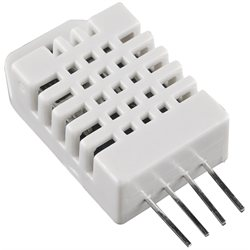
\includegraphics[scale=0.8]{./Figures/dht22.jpg}
        \rule{35em}{0.5pt}
    \caption[DHT22 sensor]{DHT22 humidity and temperature sensor.}
    \label{fig:DHT22}
\end{figure}


%------------------------------------
%	SUBSECTION 2 - MINI SOUND SENSOR
%------------------------------------

\subsection{Emartee Mini Sound Sensor}
\label{sub:sound}

Manufactured by Emartee, can also be found by the name of ``Emartee part number 4021'', and can be used to measure noise levels among other uses. Esentially, it consists on a microphone with a built-in amplifier onto a breakout board. This last feature can be useful to work directly with perfboards or breadboards\footnote{Both are construction bases for rapid prototyping of electronic circuits.}.

The output signal is analog and is increased (amplified) by some factor that allows an Arduino or any device with analog input pins to detect this signal easily\citep{gertz2012environmental}. Its operating voltage is 5V.


%------------------------------------
%	SUBSECTION 3 - SHARP DUST
%------------------------------------

\subsection{Sharp GP2Y1010AU0F}
\label{sub:sharp}

This is an inexpensive optical dust sensor, used to measure air quality. It is made out of an infrarred emitting diode which, with a well positioned phototransistor can measure the reflected IR rays thus detecting dust levels in the air\citep{sharp}. This device, which can be powered with up to 7V gives an output voltage proportional to dust density in the air. Some of its applications are air monitoring and air conditioning.

\begin{figure}[htbp]
    \centering
        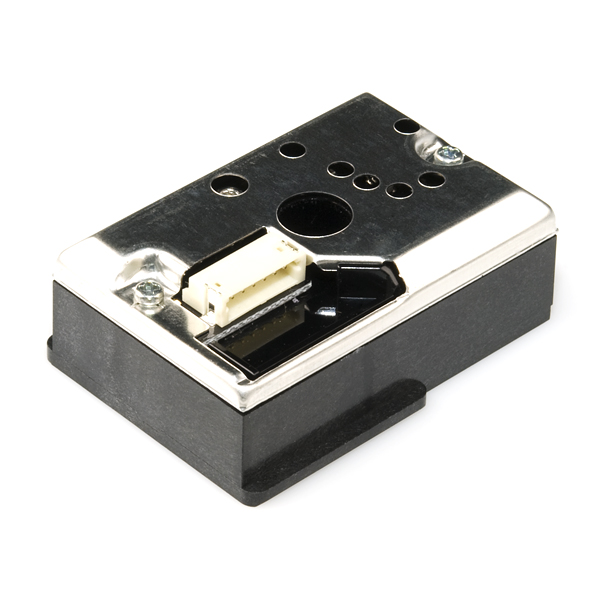
\includegraphics{./Figures/sharp.jpg}
        \rule{35em}{0.5pt}
    \caption[Sharp GP2Y1010AU0F]{Sharp GP2Y1010AU0F optical dust sensor.}
    \label{fig:SharpGP2Y1010AU0F}
\end{figure}

Surprisingly, this detector, which is priced at the time of writing about \$12, gives very precise results, similar to those offered by an expensive laser particle counter\citep{airquality}.


%-----------------------------------
%	SUBSECTION 4 - LM35
%-----------------------------------
\subsection{LM35}
\label{sub:lm35}

The LM35 is an analog sensor designed by Texas Instruments that precisely measures temperature\footnote{Datasheet: \url{http://www.ti.com/lit/ds/symlink/lm35.pdf}}. Its output is linear to temperature ---in Celsius degrees--- which means that this sensory value will not have to be processed later.

\begin{figure}[htbp]
    \centering
        \includegraphics[scale=0.6]{./Figures/LM35.jpg}
        \rule{35em}{0.5pt}
    \caption[TI LM35 temperature sensor]{TI LM35 temperature sensor.}
    \label{fig:lm35}
\end{figure}

%----------------------------------------------------------------------------------------
%	SECTION 2 - XBEE MODULE
%----------------------------------------------------------------------------------------

\section{Digi XBee\textregistered{} Wireless RF Module}
\label{sec:xbee}

These radio modules are based on the IEEE 802.15.4 standard and provide unexpensive, low power, low rate communication. They mainly use ISM\footnote{Descripción de ISM.} bands. 

\begin{figure}[htbp]
    \centering
    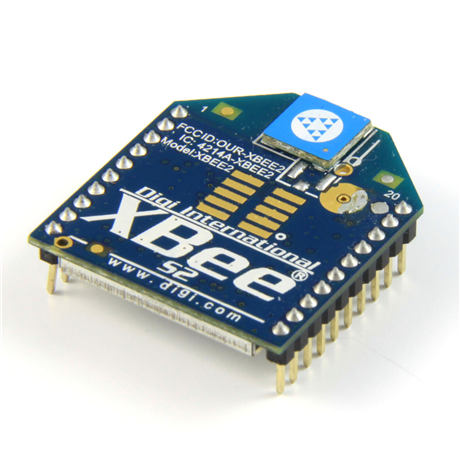
\includegraphics[scale=0.4]{./Figures/xbee.png}
        \rule{35em}{0.5pt}
        \caption[Digi XBee RF Module]{Digi XBee\textregistered{} Wireless RF Module}
    \label{fig:XBee RF Module}
\end{figure}

There are two versions of these modules, chronologically named ``Series 1'' and ``Series 2''. The older version implements the previously mentioned IEEE 802.15.4 standard which enables the network to be configured in point to point topologies. This standard specifies the physycal and media access control layers for WPANs.

On the other hand however, the latter implements a standard specification called \emph{ZigBee}\footnote{Protocol stack developed and maintained by the ZigBee Alliance. More information can be found at \url{http://zigbee.org}}. It specifies the upper layer of the protocol stack. That is, network and application layers. Although more complex, ZigBee provides mesh networking capabilities which can be a key feature in some sensor networks.

Despite their size these devices offer us many interesting features, such as 128-bit encryption, over-the-air configuration and several pins that enables the XBee to read analog values as well as working with digital input and output\citep{xbeedatasheet}.

This is why for the sake of this project ``Series 2'' has been chosen. It is worth saying that each of the two versions can transmit with different power levels thus varying the effective communication range\citep{faludi2010building}. More detailed information can be found in table \ref{tab:xbee_versions}.

Also, any XBee\textregistered{} device has two operational modes, namely transparent and API. In transparent mode ---also known as AT mode---, the device only relays serial data until it reaches the network sink. This mode is simple and ``universal'', since a connection can be established with every device that speaks and understands serial. However, neither data reception or integrity are assured (specially when working with the popular 2.4GHz ISM band, which is higly saturated) and eavesdropping can be a real problem since encryption cannot be used. 

On the other hand, API mode is slightly more complex than transparent mode, since information is encapsulated in packets. These are the main features of this operational mode:

\begin{itemize}
    \item When the sink receives a packet, it immediately transmits an ACK\footnote{Acknowledgement packets are used to indicate that the transmission was successful.} packet. If such packet is not received then transmitting radio will retry sending it.
    \item Radios can be re-configured dinamically over the air.
    \item Checksums that verify that no errors have been introduced. In other words, it checks the received information is the same than the one that was originally transmitted.
    \item Encryption (using a symmetric key algorithm) can be enabled, either using one pre-established key or getting one from the network sink.
    \item I/O samples, which enable us to use all the DIO\footnote{Although DIO stands for digital input/output, some of them can handle continous values through the ADC.} pins that the module has.
\end{itemize}

% -T-A-B-L-E---- 
\begin{table}[ht] 
\centering
\begin{tabular}{c|l l l}
    Version     & Power                 & Indoor range     & LoS range\footnotemark[7]\\
\hline
Series 1        & 1mW                   & 30m              & 100m\\
Series 1 PRO    & 63mW\footnotemark[8]  & 90m              & 1600m\\
Series 2        & 2mW                   & 40m              & 120m\\
Series 2 PRO    & 63mW\footnotemark[8]  & 90m              & 1500m\\
\end{tabular}
\caption{Comparison of different versions of XBee\textregistered.}
\label{tab:xbee_versions}
\end{table}

\footnotetext[7]{LoS range refers to line of sight range. That is, when a straight line can be drawn from the transmitter to the receiver. In this situation, there are no obstacles between them and better bitrates and/or ranges can be achieved.}
\footnotetext[8]{This output power can be obtained using high gain antennas.}

Also, if extra range is needed (up to 40km in line of sight) there are also XBee\textregistered{} devices that transmit in lower ISM bands ---900 and 868 MHz---. However, when transmitting in these frequencies neither ZigBee nor IEEE 802.15.4 can be used. DigiMesh\texttrademark{} networking protocol is the only option and it is property of Digi International Inc, which has extra features.


%----------------------------------------------------------------------------------------
%	SECTION 3 - ARDUINO
%----------------------------------------------------------------------------------------

\section{Arduino}

Arduino is the leading protopying platform nowadays. It is completely open source including the schematics of the hardware itself, which is a single-board microcontroller. Anyone can program the board through a programming language very similar to C/C++ and based on Wiring\footnote{\url{http://wiring.org.co}}. To upload a sketch ---a program--- to the microcontroller they also have developed an Arduino IDE based on the Processing IDE\footnote{More information about Processing and its IDE can be found at \url{htpp://processing.org}}.
% TODO - Check footnotes indexes

The amount of projects related to this platform is incredibly big, and it has gained huge popularity amongst designers, hackers, programmers and hobbyists these past years. It offers several advantages over similar devices, because it is really cheap, cross-platform and has every benefit inherent to the open source initiative. Also, like other open projects Arduino comes in many ``flavours'' depending on the characteristics of the project.

As it can be seen in figure \ref{fig:ArduinoUNO}, the board has many input/output pins that are compatible with analog and digital values. It's not just that but also it can establish a serial communication with a computer so interaction between programs and the platform can take place.


\begin{figure}[htbp]
    \centering
    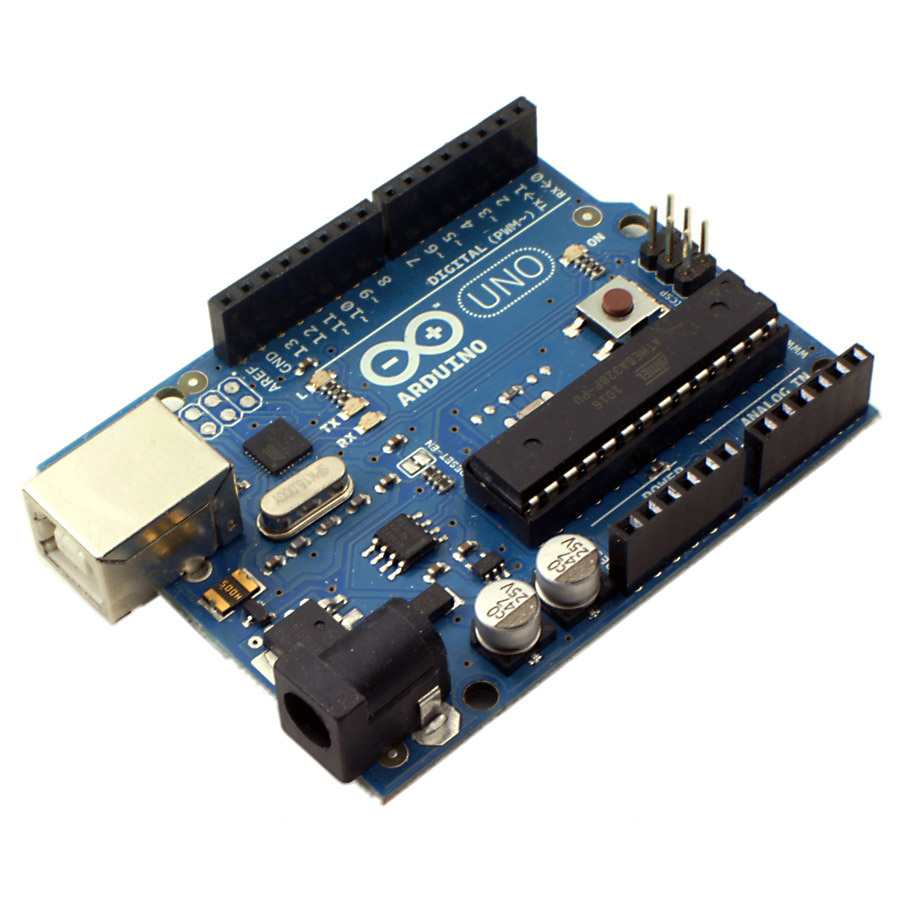
\includegraphics[scale=0.2]{./Figures/auno.jpg}
        \rule{35em}{0.5pt}
        \caption[Arduino UNO]{Arduino UNO prototyping platform.}
    \label{fig:ArduinoUNO}
\end{figure}

Arduino UNO is the one ``flavour'' that has been chosen to perform this project, since it is cheap and also the most common. That means all shields\footnote{A shield is another board plugged on top of the Arduino to extend its functionalities (for instance Ethernet, Wi-Fi, SD cards, etc.).}  work by default on it and the community it has is the biggest. In particular, this model has the following features (table \ref{tab:arduinofeatures}):
\\

\begin{table}[ht] 
\centering
\begin{tabular}{l|l}
    Feature     & Value\\
\hline
Microcontroller	& ATmega328\\
Operating Voltage &	5V\\
Input Voltage (recommended) & 7-12V\\
Input Voltage (limits) & 6-20V\\
Digital I/O Pins & 14 (of which 6 provide PWM output)\\
Analog Input Pins & 6\\
DC Current per I/O Pin & 40 mA\\
DC Current for 3.3V Pin & 50 mA\\
Flash Memory & 32 KB (ATmega328) of which 0.5 KB used by bootloader\\
SRAM & KB (ATmega328)\\
EEPROM &	1 KB (ATmega328)\\
Clock Speed &	16 MHz\\
\end{tabular}
\caption[Characteristics of the Arduino UNO]{Characteristics of the Arduino UNO. Taken from the official Arduino website (\url{http://arduino.cc}).}
\label{tab:arduinofeatures}
\end{table}

\subsection{External libraries}
In order to interact with the XBee module I used the \texttt{xbee-arduino} library, which is C/C++ library that enables an Arduino to send and receive information via an XBee\textregistered{} radio. It was originally developed by Andrew Rapp and is currently hosted on Google Code\footnote{More information can be found at \url{https://code.google.com/p/xbee-arduino/}}.


%----------------------------------------------------------------------------------------
%	SECTION 4 - RASPBERRY PI
%----------------------------------------------------------------------------------------
\section{Raspberry Pi}

\begin{figure}[htbp]
    \centering
    \includegraphics[scale=0.2]{./Figures/pi.jpg}
        \rule{35em}{0.5pt}
        \caption[Raspberry Pi]{A Raspberry Pi.}
    \label{fig:RaspberryPi}
\end{figure}

This device is an inexpensive GNU/Linux box that follows an ARM architecture and acts as the sink of the network. There are two models of this device: one that has 256MB of RAM (known as ``model A''), and another one that has 512MB of such memory (``model B''). As for the processor it utilizes a 700MHz Broadcom SoC\footnote{System on a chip are integrated circuits that collect all the necessary modules of a traditional computer in one single chip.}. The operating system is directly loaded from an SD.

Currently it supports many popular distributions, such as: Arch Linux, Raspbian (a fork of Debian specifically designed to run on the Raspberry Pi), Gentoo, NetBSD, etc.

This is an optional part of the network since an XBee can be attached to any device that speaks serial. Nonetheless it is small and low-power, providing the necessary versatility for this kind of systems.

%----------------------------------------------------------------------------------------
%	SECTION 5 - WI-FI DONGLE
%----------------------------------------------------------------------------------------
\section{D-Link DWA-123}

The Raspberry Pi, as stated before, has an ethernet interface, but in case such option is not available, a Wi-Fi dongle is the best solution. This model in particular is works out-of-the box with some Raspberry Pi GNU/Linux distributions. Also, it is cheap and supports IEEE 802.11b/g/n. This device will be the bridge between the XBee network and the Internet.


%----------------------------------------------------------------------------------------
%	SECTION 6 - Arch GNU/Linux ARM
%----------------------------------------------------------------------------------------
\section{Arch Linux ARM}
\label{sec:alarmmm}

The project originally started as a port of the popular distribution Arch Linux\footnote{\url{http://archlinux.org}}, compiled for ARM devices. The main feature of this ``distro'' is \emph{simplicity}.

\begin{figure}[htbp]
    \centering
    \includegraphics[scale=0.4]{./Figures/alarm.png}
        \rule{35em}{0.5pt}
        \caption[Arch Linux ARM Logo]{Arch Linux ARM logo.}
    \label{fig:alarm_logo}
\end{figure}

Arch Linux ARM follows, as its predecessor does, the KISS (``keep it simple, stupid'') principle, which means it just provides a working and minimalist system to work with. That is, no unnecessary packages are installed by default, giving the user complete control of its operative system. For instance, no GUI is available by default and everything must be done through the terminal (at least in the first place). This means the Raspberry Pi will be running a lightweight operative system, therefore leaving more resources to process all the data.


%----------------------------------------------------------------------------------------
%	SECTION 7 - Python
%----------------------------------------------------------------------------------------
\section{Python}
\label{sec:whatispython}

Python is a general-purpose, high-level scripting programming language that first saw the light of day in 1991, originally designed by Guido van Rossum. It is an open source language that has more than one implementation. The default implementation ---and used in this project--- is CPython, which is written in C. 

There are two main versions of this programming language, 2.x and 3.x which are not compatible. Version 2.x will be the one used to complete the project since more libraries and modules use Python 2.x.

\begin{figure}[htbp]
    \centering
    \includegraphics[scale=0.4]{./Figures/python-logo.png}
        \rule{35em}{0.5pt}
        \caption[Python logo]{Python logo.}
    \label{fig:pythonlogo}
\end{figure}

This project does not utilize solely the standard libraries but also some additional ones, such as:

\begin{itemize}
    \item \texttt{pyserial}\footnote{\url{http://pyserial.sourceforge.net/}} --- This library enables Python to establish serial connections (more specifically, following the RS-232 standard) with all kinds of devices. In this case, it allows us to receive data from an XBee\textregistered{} module.
    \item \texttt{python-xbee}\footnote{\url{https://code.google.com/p/python-xbee/}} --- Written by Paul Malmsten, this library allows Python to work with XBee API serial information. It has two main operational modes, synchronous and asynchronous. That is, continuously receiving information from an XBee\textregistered{} (and blocking the whole program until it finishes) or spawning a new background thread every time a new packet arrives, respectively.
    \item \texttt{python-requests}\footnote{\url{http://python-requests.org/}} --- This is an HTTP library that, according to its creator, is written ``for human beings''. In other words, HTTP requests made easy. This module will be used to upload sensory data to the Internet
\end{itemize}
